\documentclass[12pt]{article} %V1.0
\usepackage{amsfonts,amssymb,amsmath,mathrsfs,amsthm}
\usepackage{graphicx,caption,lipsum}
\usepackage{epsfig,epstopdf}
%\usepackage{harvard}

%\usepackage[margin=2cm]{geometry}
\usepackage[bottom=1in,top=1in,left=1in,right=1in]{geometry}
\setlength{\parindent}{0cm}

%\setlength{\leftmargini}{16pt}

\usepackage[dvipsnames]{xcolor} % en.wikibooks.org/wiki/LaTeX/Colors
\usepackage{enumitem} % bullet points
\usepackage{cmap} % fix the 'fi' problem
\usepackage{rotating,wrapfig,lscape}
\usepackage{bbm}
\usepackage{mathtools} % for multi-lined equations
\usepackage[utf8]{inputenc}
\usepackage[english]{babel}

\usepackage[export]{adjustbox}
\usepackage{setspace}

\onehalfspacing



\newtheorem{theorem}{Theorem}
\newtheorem{corollary}{Corollary}[theorem]
\newtheorem{lemma}[theorem]{Lemma}
\newtheorem{proposition}{Proposition}
 

\linespread{1.25}
\setlength{\parindent}{24pt}



% HYPERLINK
\usepackage[breaklinks=true]{hyperref}
\hypersetup{
  colorlinks=true,
  citecolor=darkblue,
  linkcolor=darkblue,
  urlcolor=darkblue,
  pdfpagemode=none,
  pdfstartview={XYZ null null 1},
  pdftitle={},
  pdfauthor={GH},
  pdfkeywords={} }
\definecolor{darkblue}{rgb}{0,0,0.25}
%
% BIBLIOGRAPHY
\usepackage[longnamesfirst]{natbib}
\bibliographystyle{chicago}
%\bibliographystyle{econometrica}

% DEFINITIONS
\theoremstyle{definition}
\newtheorem{definition}{Definition}%[section]

\captionsetup[figure]{labelsep=period}

\usepackage{palatino}

\setlength{\footnotesep}{1em}

\usepackage{nameref}

\graphicspath{{./figs181014/}}
%---------------------------------------------------------------------------------

\begin{document}

%---------------------------------------------------------------------------------

\section{Appendix: No Scar}\label{section appendix no scar}
In the main part of this paper, we worked with the ``model with skill loss \textbf{and} scar" in which young workers who stay unemployed for a prolonged period of time if hit by a skill loss shock get permanently scarred affecting their productivity for their lifetime. Here, we present the version of the ``model with skill loss \textbf{but without any} scar". All the variables and parameters are similar to the main model except the key difference that the skill loss does not scar the workers permanently; once they have been employed at least once and then lose their job, all types of workers end up in the same pool of unemployed workers ($u_1$ in the below figure) and have no permanent difference in productivity.
\begin{figure}[h]
	\centering
	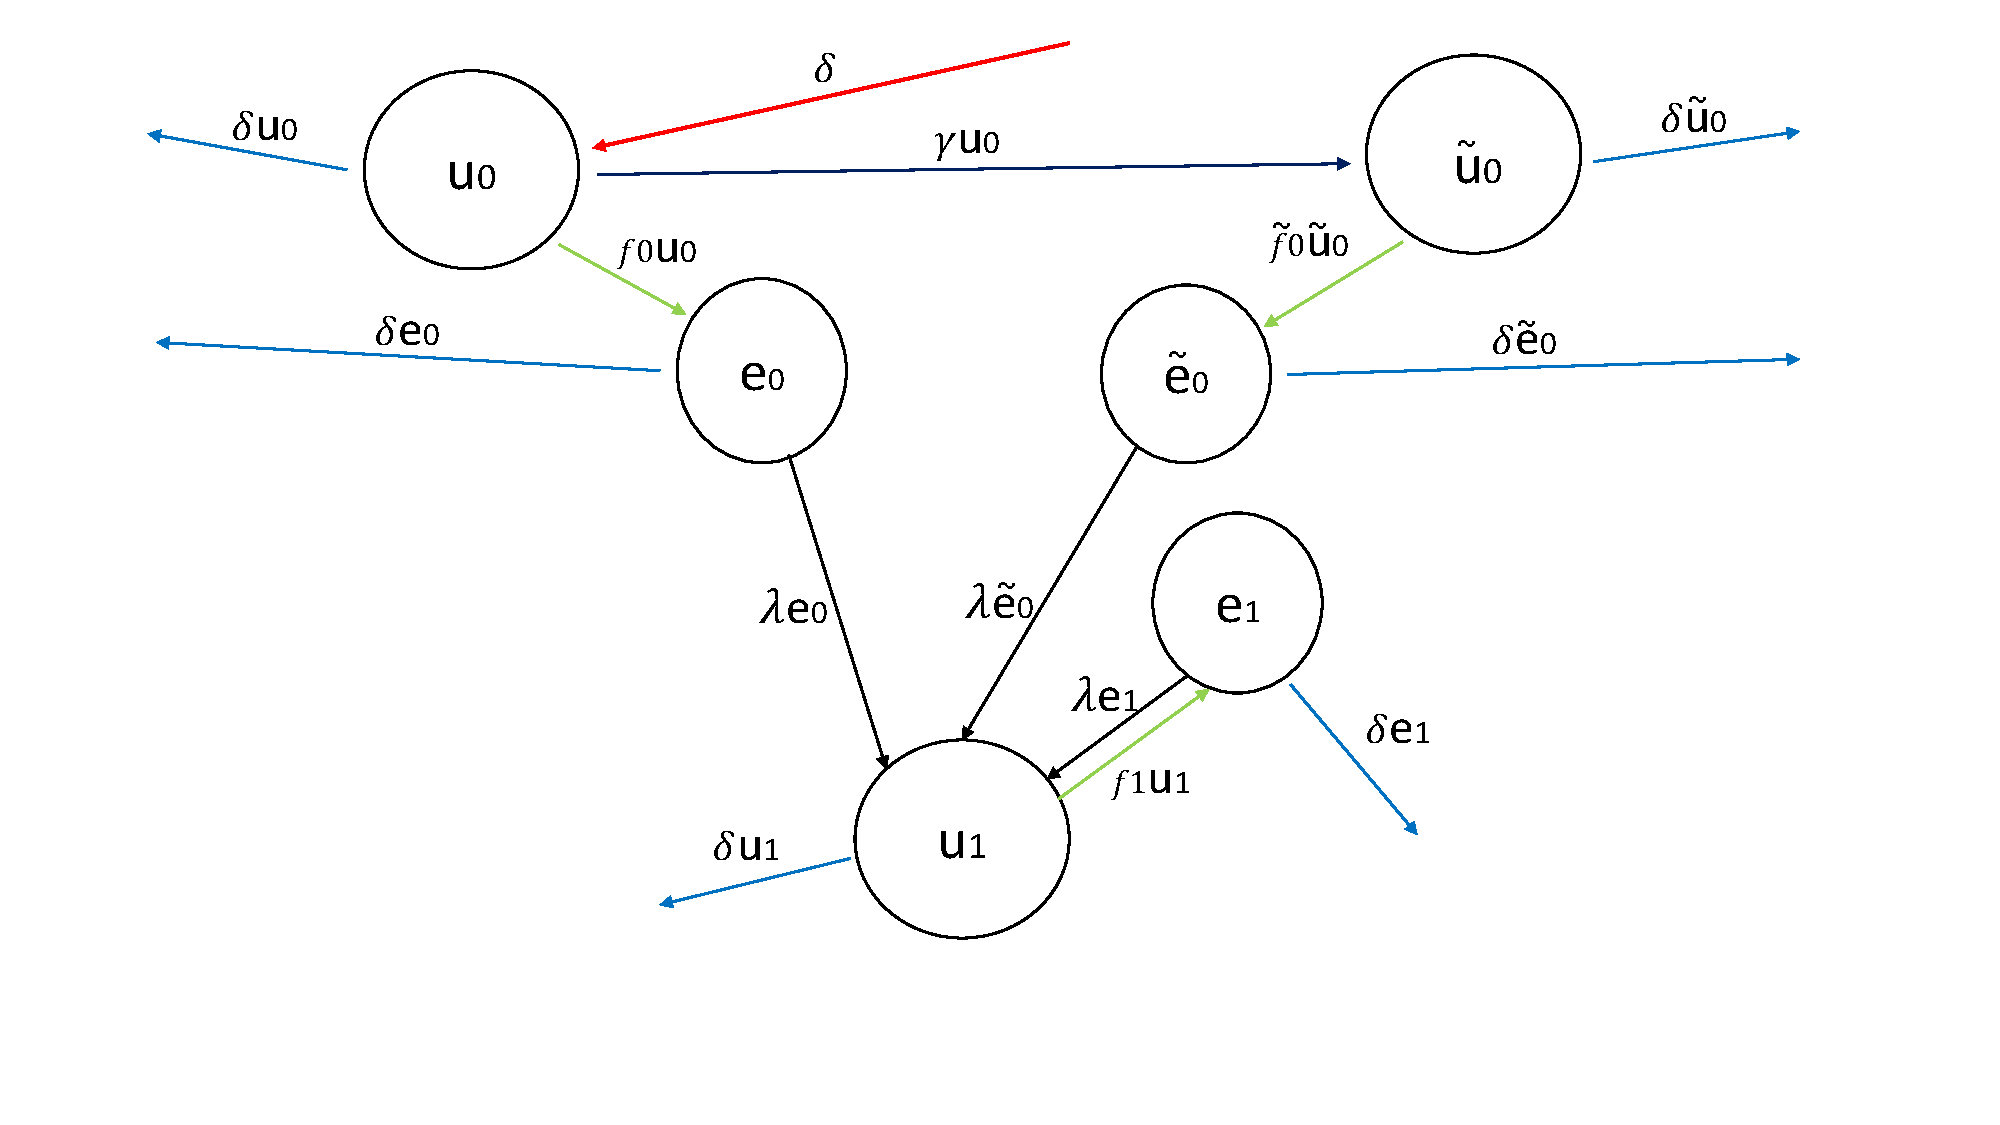
\includegraphics[width=1.05\linewidth]{empl_states_no_scar.pdf}
	\vspace{0em}
	\caption{Worker flows in and out of the various states (model with no scar).}
	\label{figure model no scar}
\end{figure}
\subsection{Beveridge curves}\label{section beveridge no scar}
To derive the Beveridge curves, we can look at above figure, which illustrates the worker flows in and out of every state in the environment without any scar. The graph is a simplified version of figure 1, so the interpretation is similar. 

Equating the flows in and out of the various states and after some algebra, we find the following steady state measure of workers in the various states:   
\begin{eqnarray*}
u_0 &=& \frac{\delta}{\delta+\gamma+f_0},  \\
\tilde{u_0} &=& \frac{\gamma}{\delta+\Tilde{f_0}} \cdot  \frac{\delta}{\delta+\gamma+f_0},   \\
u_1 &=& \frac{\lambda(\gamma\Tilde{f_0}+\delta f_0 + f_0\Tilde{f_0})}{(\delta+\Tilde{f_0})(\delta+\gamma+f_0)(\delta + \lambda + f_1)} , \\
e_0 &=& \frac{f_0}{\delta+\lambda} \cdot \frac{\delta}{\delta+\gamma+f_0}, \\
\Tilde{e_0} &=& \frac{\Tilde{f_0}}{\delta+\lambda} \cdot \frac{\gamma}{\delta + \Tilde{f_0}} \cdot \frac{\delta}{\delta+\gamma+f_0},  \\
 e_1 &=& \frac{f_1}{\delta+\lambda} \cdot \frac{\lambda(\gamma\Tilde{f_0}+\delta f_0 + f_0\Tilde{f_0})}{(\delta+\Tilde{f_0})(\delta+\gamma+f_0)(\delta + \lambda + f_1)} . 
\end{eqnarray*}

\subsubsection{Value Functions}\label{section value functions no scar}
Next, we find the steady state value functions similar to before. We start with a vacant firm with $q$ as its arrival rate of workers to firms:
\begin{equation*}
   rV = -c + q_0 (J_0-V) + \Tilde{q_0}(\Tilde{J_0}-V) + q_1 (J_1-V).
\end{equation*}The free entry implies that $V=0$ in equilibrium, so, the above free entry condition becomes 
\begin{equation}
   c = q_0J_0 + \Tilde{q_0}\Tilde{J_0} + q_1J_1.\label{eq free entry no scar} 
\end{equation}

We have three value functions for productive firms in the various states, i.e., for firms who matched with the three different types of workers (type 0, $\tilde{0}$, and 1). 

\begin{eqnarray}
     rJ_0 &=& p-\kappa-w_0-\lambda J_0 - \delta J_0, \label{eq J0 no scar} \\
     r\Tilde{J_0} &=& p-\Tilde{\kappa}-\Tilde{w_0}-\lambda \Tilde{J_0} - \delta \Tilde{J_0}, \label{eq J0 tilde no scar} \\
    rJ_1 &=& p-w_1-\lambda J_1 - \delta J_1. \label{eq J1 no scar} 
    \end{eqnarray}

Now, we move on to the value functions of workers in the various states. All the notations are standard. The value functions for unemployed workers in the various states are given by: 
\begin{eqnarray}
    rU_0 &=& z+f_0(W_0-U_0)+\gamma(\Tilde{U_0}-U_0) - \delta U_0, \label{eq U0 no scar} \\
     r\Tilde{U_0} &=& z+\Tilde{f_0}(\Tilde{W_0}-\Tilde{U_0})- \delta \Tilde{U_0},
     \label{eq U0 tilde no scar} \\
    rU_1 &=& z+f_1(W_1-U_1)- \delta U_1. \label{eq U1 no scar} 
\end{eqnarray}
The value functions for employed workers in the various states are given by: 
\begin{eqnarray}
    rW_0 &=&w_0+\lambda(U_1-W_0)- \delta W_0, \label{eq W0 no scar} \\
     r\Tilde{W_0} &=& \Tilde{w_0}+\lambda(U_1-\Tilde{W_0})- \delta \Tilde{W_0},  \label{eq W0 tilde no scar} \\
     rW_1 &=& w_1+\lambda(U_1-W_1)- \delta W_1. \label{eq W1 no scar} 
     \end{eqnarray}
Similar to before any inexperienced workers who lose their first job move to the pool of experienced unemployed workers, so the term $U_1$ appears on the right-hand side of equations for $W_0$ and $\Tilde{W_0}$.

Now, we have all the value functions for the firms and workers, we can move to the bargaining problems in the various types of meetings in this environment without any scar. 

\subsubsection{Bargaining problems}\label{section bargaining no scar} 
\textbf{Bargaining in type-1 meeting}

\medskip 

\noindent Like in the case for the model with scar, solving the standard Nash bargaining problem between a firm and an unemployed worker of type-1 implies that the following condition must be satisfied:
\begin{equation}
(1-\eta)(W_1-U_1) = \eta J_1. \label{eq bargain 1 no scar}
\end{equation}
Following similar steps as before, we use the value functions for $W_1$, $J_1$, and $U_1$ from (\ref{eq W1 no scar}, \ref{eq J1 no scar}, and \ref{eq U1 no scar} respectively) to get the following equation for the ``wage curve" for type-1 workers in this environment with no scar. 
\begin{equation}
 w_1 = \frac{\eta p (r+\lambda+\delta+f_1)+(1-\eta)z(r+\lambda+\delta)}{r+\lambda+\delta + \eta f_1}. \label{eq WC1 no scar}
\end{equation} Note that the equation is identical to wage curve in the model with scar. 

\bigskip 

\noindent \textbf{Bargaining in type-$\Tilde{0}$ meeting}

\medskip 

\noindent The surplus sharing rule between an inexperienced worker who suffered skill loss and a firm is given by the following equation:
\begin{equation}
       (1-\eta)(\Tilde{W_0}-\Tilde{U_0}) = \eta \Tilde{J_0}.  \label{eq bargain 0 tilde no scar}
\end{equation}Same as before, we replace the value functions $\tilde{W_0}$ and $\tilde{J_0}$ from (\ref{eq W0 tilde no scar}) and (\ref{eq J0 tilde no scar}), respectively, to write the wage of a type-$\tilde{0}$ worker as
\begin{equation}
   \Tilde{w_0} = \eta (p-\Tilde{\kappa})  - \lambda (1-\eta)(U_1 - \Tilde{U_0}) + (1-\eta)(r+\delta) \Tilde{U_0} . \label{eq w0 tilde first step no scar}
    \end{equation}
    
Notice that $U_1-\Tilde{U_0}$ appears in the above equation, so we need to subtract (\ref{eq U0 tilde no scar}) from (\ref{eq U1 no scar}) to obtain 
\begin{equation}
(U_1-\Tilde{U_0}) = \frac{f_1(W_1-U_1) - \Tilde{f_0}(\Tilde{W_0}-\Tilde{U_0})}{r+\delta}.\label{eq U1 tilde-U0 tilde no scar}
    \end{equation}
We need to substitute equations  for $U_1$, $W_1$, $\Tilde{U_0}$, and $\Tilde{U_0}$ using (\ref{eq U1 no scar}), (\ref{eq W1 no scar}), (\ref{eq U0 tilde no scar}), and (\ref{eq W0 tilde no scar}) respectively followed by some algebra to get the following wage curve for the type-$\Tilde{0}$ worker: 
    \begin{equation} 
\Tilde{w_0} = \frac{1}{r+\delta+\eta \Tilde{f_0}}\left[\eta\textcolor{red}{(p-\Tilde{\kappa})}(r+\delta+ \Tilde{f_0})+\frac{(r+\delta+\lambda)(r+\delta+f_1)}{r+\delta+\lambda+f_1}(1-\eta)z - \frac{\lambda(1-\eta)f_1}{r+\delta+\lambda+f_1}w_1 \right]. \label{eq WC0 tilde no scar}
\end{equation}

Notice that the equation is pretty similar to the wage $\Tilde{w_0}$ in the main model with scar, the only difference is that the first term now has $(p-\Tilde{\kappa})$ instead of $(p-\kappa-\Tilde{\kappa})$; the intuition is that the productivity loss is not permanent in the model without scar so the term $\kappa$ is not subtracted from the productivity term. Also, similar to the baseline model, the wage $\Tilde{w_0}$ depends on the wage that type-1 workers make. The intuition is similar to before: a type-$\tilde{0}$ worker is willing to accept a wage lower than the wage $w_1$  to get out of the ``inexperienced" state once and for all. 

\bigskip 
    
\noindent \textbf{Bargaining in type-0 meeting}

\medskip 

\noindent Finally, the bargaining problem between an unskilled worker who has not been hit by the skill loss shock and a firm is given by the following equation: 
\begin{equation}
       (1-\eta)(W_0-U_0) = \eta J_0 .  \nonumber 
\end{equation}Following standard steps, substitute ${W_0}$ and ${J_0}$ from (\ref{eq W0 no scar}) and (\ref{eq J0 no scar}), respectively, to write the wage of a type-0 worker as
\begin{equation}
    w_0 = \eta(p-\kappa) - (1-\eta)\lambda(U_1 - U_0) + (1-\eta)(r+\delta) U_0. \nonumber 
    \end{equation}
    
Similar to the case of type-$\tilde{0}$ workers, the wage for type-0 also depends on ${U_1}-{U_0}$. We follow pretty much the same steps as in the case of type-$\tilde{0}$ to get the following final formula:  
\begin{equation}
    \begin{multlined}
    w_0 = \frac{r+\delta+\gamma +f_0}{r+\delta+\gamma+\eta f_0}\eta (p-\kappa) + \frac{(r+\lambda+\delta)(r+f_1+\delta)(r+\gamma+\delta)}{(r+\delta)(r+\delta+\gamma + \eta f_0)(r+\lambda+\delta+f_1)} (1-\eta) z + \\  
\frac{\gamma \eta \Tilde{f_0}}{(r+\delta)(r+\delta+\gamma + \eta f_0)}\textcolor{red}{(p-\Tilde{\kappa}-\Tilde{w_0})}- \frac{(1-\eta)\lambda f_1 (r+\gamma+\delta)}{(r+\delta)(r+\delta+\gamma + \eta f_0)(r+\lambda+\delta+f_1)} w_1
    \end{multlined}  \label{eq WC0 no scar} 
\end{equation}

Like type-$\tilde{0}$ workers, the equation is similar to the the wage $w_0$ in the baseline model with scar. Notably, the omission of $\kappa$ from the productivity term is due to the temporary nature of skill loss. Also, type-0 workers' wage relies on both ${w_1}$ and $\tilde{w_0}$, as explained in the baseline model with scar. Her readiness to accept $w_0$ below $w_1$ reflects her desire to exit the inexperienced workforce permanently, explaining the appearance of $w_1$ in the equation. Accepting the job shields the worker from skill loss shocks, so her potential earnings if she declined the firm's offer ($\tilde{w_0}$) influence the current negotiated wage through her external option.  


\subsection{Definition of Steady State Equilibrium}\label{section definition of equil} 

\begin{definition}\label{definition equilibrium no scar}
    A steady state equilibrium in the model without scar is a list of wages for the three types of workers $(w_0, \Tilde{w_0}, w_1)$, a market tightness $\theta$, and measures of unemployed and employed workers in the various states $(u_0, \Tilde{u_0}, u_1, e_0, \Tilde{e_0}, e_1)$. The three equilibrium wages and the market tightness are the four ``core variables", which satisfy the free entry condition (\ref{eq free entry no scar}), and the three wage curves (\ref{eq WC1 no scar}), (\ref{eq WC0 tilde no scar}), and (\ref{eq WC0 no scar}). Once these core variables have been determined, the various equilibrium measures of unemployed and employed workers follow directly from the Beveridge curves derived at the end of Section \ref{section beveridge no scar}.  
\end{definition} 



%---------------------------------------------------------------------------------


%---------------------------------------------------------------------------------

\section{Government Interventions}
We explore the same three interventions, namely ``Unbiased matching", ``Government subsidies", and ``Internships", in this new environment without scar. As described earlier, each intervention will allow firms to hire inexperienced workers at lower salaries, lowering the bias against these workers and mitigating the inefficiency. 

\subsection{Intervention 1: Unbiased matching}\label{section unbiased matching}

\textbf{Beveridge Curves} 

\noindent Under this intervention, it is illegal to discriminate amongst workers, so all workers match with firms at the same rate. The Beveridge curves are same as in the Section \ref{section beveridge no scar}, but now $f_0=\Tilde{f_0}=f_1=f$.  

\bigskip 

\noindent \textbf{Value Functions}

\noindent Since the match is unbiased, the probability that a firm meets a specific a worker of a specific type depends only on that type's relative representation in the pool of unemployed. If $q$ is the arrival rate of any worker to the typical firm, the value function of a vacant firm becomes
\begin{equation}
   rV = -c + q \left[\frac{u_0}{u}(J_0-V) + \frac{\Tilde{u_0}}{u}(\Tilde{J_0}-V) + \frac{u_1}{u}(J_1-V) \right].\nonumber 
\end{equation} In equilibrium, the free entry implies $V=0$, so the free entry condition becomes
\begin{equation}
 c = \frac{q}{u} \left({u_0} J_0 + \Tilde{u_0} \Tilde{J_0} + {u_1} J_1 \right).\label{eq free entry intervention 1 no scar} 
\end{equation}

As discussed before, the process through which firms meet workers is different compared to the model without any intervention but once a firm meets a specific type of worker, the value functions for productive firms and employed workers in the various states remain the same, i.e., they are still given by equations (\ref{eq J0 no scar})-(\ref{eq J1 no scar}) and (\ref{eq W0 no scar})-(\ref{eq W1 no scar}) respectively. 

The value functions for unemployed workers in the various states are also almost identical to those in the model without intervention but with the key difference that all the arrival rates are now replaced by the common rate $f$.
\begin{eqnarray*}
    rU_0 &=& z+f(W_0-U_0)+\gamma(\Tilde{U_0}-U_0) - \delta U_0, \\
    r\Tilde{U_0} &=& z+f(\Tilde{W_0}-\Tilde{U_0})- \delta \Tilde{U_0}, \\
    rU_1 &=& z+f(W_1-U_1)- \delta U_1.
\end{eqnarray*}

\smallskip 

\noindent \textbf{Bargaining problems}

\noindent As discussed before, the intervention with unbiased matching process affects only the parts of the analysis that take place before a firm matches with a worker, so all the wage curves are identical to the model without any intervention once one has replaced the various $f$'s with the common arrival rate $f$, i.e.  
\begin{equation}
 w_1 = \frac{\eta p (r+\lambda+\delta+f)+(1-\eta)z(r+\lambda+\delta)}{r+\lambda+\delta + \eta f}. \label{eq WC1 inter 1 no scar}
\end{equation}
\begin{equation} 
\Tilde{w_0} = \frac{1}{r+\delta+\eta {f}}\left[\eta(p-\Tilde{\kappa})(r+\delta+ {f})+\frac{(r+\delta+\lambda)(r+\delta+{f})}{r+\delta+\lambda+{f}}(1-\eta)z - \frac{\lambda(1-\eta){f}}{r+\delta+\lambda+{f}}\Tilde{w_1} \right] \label{eq WC0 tilde inter 1 no scar}
\end{equation}
\begin{equation}
    \begin{multlined}
         w_0 = \frac{r+\delta+\gamma +f}{r+\delta+\gamma+\eta f}\eta (p-\kappa) + \frac{(r+\lambda+\delta)(r+f+\delta)(r+\gamma+\delta)}{(r+\delta)(r+\delta+\gamma + \eta f)(r+\lambda+\delta+f)} (1-\eta) z \label{eq WC0 inter 1} \\  
+ \frac{\gamma {f}}{(r+\delta)(r+\delta+\gamma + \eta f)}\eta(p-\Tilde{\kappa}-\Tilde{w_0}) - \frac{(1-\eta)\lambda f (r+\gamma+\delta)w_1}{(r+\delta)(r+\delta+\gamma + \eta f)(r+\lambda+\delta+f)}.
    \end{multlined} \label{eq WC0 inter 1 no scar}
\end{equation}

\bigskip 

\begin{definition}\label{definition equil inter 1 no scar}
    A steady state equilibrium for the model without scar, under Intervention 1, is a list of wages for the three types of workers $(w_0, \Tilde{w_0}, w_1)$, a market tightness $\theta$, and measures of unemployed and employed workers in the various states $(u_0, \Tilde{u_0}, u_1, e_0, \Tilde{e_0}, e_1)$. The three equilibrium wages and the market tightness are the four ``core variables", which satisfy the free entry condition (\ref{eq free entry intervention 1 no scar}), and the three wage curves (\ref{eq WC1 inter 1 no scar}), (\ref{eq WC0 tilde inter 1 no scar}), and (\ref{eq WC0 inter 1 no scar}). Once these core variables have been determined, the various equilibrium measures of unemployed and employed workers follow directly from the Beveridge curves, after one replaces the various $f$'s with the common arrival rate $f$.
\end{definition} 

%---------------------------------------------------------------------------------
\section{Government Interventions}
\subsection{2A: Illegal to bias}
All the Beveridge curves the same with $f_0=\Tilde{f_0}=f_1=f$.
\subsubsection{Beveridge curves}
Equating the inflow and outflow of $u_0$:
\begin{equation}
    \delta = u_0(\delta+\gamma+f) \\
    \implies u_0 = \frac{\delta}{\delta+\gamma+f}
\end{equation}
Equating the inflow and outflow of $\Tilde{u_0}$:
\begin{equation}
    \gamma u_0 = \Tilde{u_0}(\delta+f) \\
    \implies \Tilde{u_0} = \frac{\gamma}{\delta+f} \cdot \frac{\delta}{\delta+\gamma+f}
\end{equation}
Equating the inflow and outflow of $u_1$:
\begin{align*}
    \gamma (\delta + f)u_1 &= \lambda e = \lambda (1-u_0-\Tilde{u_0}-u_1)\\
    \implies u_1(\delta + \lambda + f) &= \lambda \left[ 1 -\frac{\delta}{\delta+\gamma+f} - \frac{\gamma}{\delta+\Tilde{f}} \cdot \frac{\delta}{\delta+\gamma+f}\right] \\
    &= \lambda \left[ 1 -\frac{\delta}{\delta+\gamma+f} \left(\frac{\delta+f+\gamma}{\delta+f}\right)\right] \\
     &= \lambda \left[ \frac{\delta^2 + \delta f + \gamma \delta + \gamma f_0 + \delta f + f^2 - \delta^2 - \delta f-\delta \gamma}{(\delta+f)(\delta+\gamma+f)} \right] \\
     &= \frac{\lambda f(\gamma + f +\delta)} {(\delta+f)(\delta+\gamma+f)(\delta + \lambda + f)} 
\end{align*}
\begin{equation}
    \therefore u_1 = \frac{\lambda f}{(\delta+f)(\delta + \lambda + f)} 
\end{equation}

Equating the inflow and outflow of $e_0$:
\begin{equation}
    e_0(\delta + \lambda) = f u_0 \\
    \implies e_0 = \left(\frac{f}{\delta+\lambda}\right) \cdot \left(\frac{\delta}{\delta+\gamma+f}\right) 
\end{equation}

Equating the inflow and outflow of $\Tilde{e_0}$:
\begin{equation}
    \Tilde{e_0}(\delta + \lambda) = f\Tilde{u_0} \\
    \implies \Tilde{e_0} = \left(\frac{f}{\delta+\lambda}\right) \cdot \left(\frac{\gamma}{\delta + f}\right) \cdot \left(\frac{\delta}{\delta+\gamma+f}\right) 
\end{equation}

Equating the inflow and outflow of $e_1$:
\begin{equation}
    e_1(\delta + \lambda) = f u_1 \\
    \implies e_1 = \left(\frac{f}{\delta+\lambda}\right) \cdot \left(\frac{\lambda f}{(\delta+f)(\delta + \lambda + f)} \right) 
\end{equation}
\subsubsection{Value Functions}

\begin{equation}
    c = q \frac{u_0}{u}J_0 + q \frac{\Tilde{u_0}}{u} \Tilde{J_0} + q \frac{u_1}{u}J_1
\end{equation}

\begin{equation}
    rJ_0 =p-\kappa-w_0-\lambda J_0 - \delta J_0 \implies J_0 = \frac{p-
    \kappa-w_0}{r + \lambda + \delta}
\end{equation}

\begin{equation}
    r\Tilde{J_0} =p-\Tilde{\kappa}-\Tilde{w_0}-\lambda \Tilde{J_0} - \delta \Tilde{J_0} \implies \Tilde{J_0} = \frac{p-\Tilde{\kappa}-\Tilde{w_0}}{r + \lambda + \delta}
\end{equation}

\begin{equation}
    rJ_1 =p-w_1-\lambda J_1 - \delta J_1 \implies J_1 = \frac{p-w_1}{r + \lambda + \delta}
\end{equation}

\begin{equation}
    rU_1 =z+f(W_1-U_1)- \delta U_1 \implies U_1 = \frac{z + f W_1}{r + \delta + f}
\end{equation}

\begin{equation}
    rU_0 =z+f(W_0-U_0)+\gamma(\Tilde{U_0}-U_0) - \delta U_0 \implies U_0 = \frac{z + f W_0 + \gamma \Tilde{U_0}}{r + \gamma + \delta + f}
\end{equation}

\begin{equation}
    r\Tilde{U_0} =z+f(\Tilde{W_0}-\Tilde{U_0})- \delta \Tilde{U_0} \implies \Tilde{U_0} = \frac{z + f\Tilde{W_0}}{r + \delta + f}
\end{equation}

\begin{equation}
    rW_1 =w_1+\lambda(U_1-W_1)- \delta W_1 \implies W_1 = \frac{w_1 + \lambda U_1}{r + \delta + \lambda}
\end{equation}

\begin{equation}
    rW_0 =w_0+\lambda(U_1-W_0)- \delta W_0 \implies W_0 = \frac{w_0 + \lambda U_1}{r + \delta + \lambda}
\end{equation}

\begin{equation}
    r\Tilde{W_0} =\Tilde{w_0}+\lambda(U_1-\Tilde{W_0})- \delta \Tilde{W_0} \implies \Tilde{W_0} = \frac{\Tilde{w_0} + \lambda U_1}{r + \delta + \lambda}
\end{equation}

\subsubsection{Bargaining problems}
\textbf{Bargaining in type-1 meeting}
\begin{align*}
    (1-\eta)(W_1-U_1) &= \eta J_1 \\
     \implies (1-\eta) \left[ \frac{w_1 + \lambda U_1 - rU_1-\delta U_1 - \lambda U_1}{r+\lambda + \delta}\right] &= \eta \frac{p-w_1}{r+\lambda+\delta} \\
    \implies w_1 &= \eta p + (1-\eta)(r+\delta)U_1 \\
   &= \eta p + (1-\eta)z + (1-\eta)f(W_1-U_1) \\
   &= \eta p + (1-\eta)z + \eta f J_1 \\
   &= \eta p + (1-\eta)z + \eta f \frac{p-w_1}{r+\lambda +\delta} \\ 
   \implies w_1\left(\frac{r+\lambda+\delta+\eta f}{r+\lambda+\delta}\right) &= \eta p \left(\frac{r+\lambda+\delta+f}{r+\lambda+\delta}\right) + (1-\eta)z
\end{align*}
\begin{equation}
    \therefore w_1 = \left(\frac{r+\lambda+\delta+f}{r+\lambda+\delta+\eta f}\right) \eta p + \left(\frac{r+\lambda+\delta}{r+\lambda+\delta+\eta f}\right) (1-\eta)z
\end{equation}

\textbf{Bargaining in type-$\Tilde{0}$ meeting}
\begin{align*}
    (1-\eta)(\Tilde{W_0}-\Tilde{U_0}) &= \eta \Tilde{J_0} \\
     \implies (1-\eta) \left[ \frac{\Tilde{w_0} + \lambda(U_1 - \Tilde{U_0}) - (r+\delta)\Tilde{U_0}}{r+\lambda+\delta}\right] &= \eta \frac{p-\Tilde{w_0}-\Tilde{\kappa}}{r+\lambda+ \delta}   \\
    \implies \Tilde{w_0} +  \lambda (1-\eta)(U_1 - \Tilde{U_0}) - (1-\eta)(r+\delta) \Tilde{U_0} &= \eta (p-\Tilde{\kappa}) 
\end{align*}
\begin{equation}
    \Tilde{w_0} = \eta (p-\Tilde{\kappa})+ (1-\eta)(r+\delta) \Tilde{U_0} - \lambda (1-\eta)(U_1 - \Tilde{U_0}) 
\end{equation}
From the value functions:
\begin{align*}
    \Tilde{U_0} &= \frac{z + f (\Tilde{W_0}-\Tilde{U_0})}{r+\delta} \\
    (U_1-\Tilde{U_0}) &= \frac{f[(W_1-U_1) -(\Tilde{W_0}-\Tilde{U_0})]}{r+\delta} \\
    (W_1-U_1) &= \frac{w_1-z}{r+\delta+\lambda+f} 
\end{align*}
Now, going back to (39),
\begin{align*}
     \Tilde{w_0} &= \eta(p-\Tilde{\kappa}) + (1-\eta)[z + f(\Tilde{W_0}-\Tilde{U_0})] - \frac{\lambda (1-\eta)f}{r+\delta}\left[\frac{w_1-z}{r+\delta+\lambda+f}  -(\Tilde{W_0}-\Tilde{U_0})\right] \\
     &= \eta(p-\Tilde{\kappa}) + (1-\eta)z + f(1-\eta)(\Tilde{W_0}-\Tilde{U_0})\left[1+\frac{\lambda}{r+\delta}\right] - \frac{\lambda (1-\eta)f}{r+\delta}\frac{w_1-z}{r+\delta+\lambda+f}\\
     &= \eta(p-\Tilde{\kappa}) + (1-\eta)z\left[\frac{(r+\lambda+\delta)(r+f+\delta)}{(r+\delta)(r+\lambda+\delta+f)}\right] + \eta f \Tilde{J_0} \frac{(r+\lambda+\delta)}{r+\delta} - \\ & \frac{\lambda (1-\eta)f w_1}{(r+\delta)(r+\delta+\lambda+f)}\\
    \Tilde{w_0}\left(\frac{r+\delta+\eta f}{r+\delta}\right) &= \eta(p-\Tilde{\kappa}) \left(\frac{r+\delta+f}{r+\delta}\right) + (1-\eta)z\frac{(r+\delta+\lambda)(r+\delta+f)}{(r+\delta)(r+\delta+\lambda+f)}-\frac{\lambda(1-\eta)fw_1}{(r+\delta)(r+\delta+\lambda+f)}
\end{align*}
\begin{equation}
    \therefore \Tilde{w_0} = \frac{1}{r+\delta+\eta f}\left[\eta(p-\Tilde{\kappa})(r+\delta+f)+(1-\eta)z\frac{(r+\delta+\lambda)(r+\delta+f)}{r+\delta+\lambda+f} - \frac{\lambda(1-\eta)f}{r+\delta+\lambda+f}w_1 \right]\\
\end{equation}
\textbf{Bargaining in type-0 meeting}
\begin{align*}
    (1-\eta)(W_0-U_0) &= \eta J_0 
    \\
     \implies (1-\eta)\frac{w_0 + \lambda U_1 -(r+\delta-\lambda)U_0}{r+\lambda+\delta} &= \eta \frac{p-w_0-\kappa}{r+\lambda+\delta}   \\
    \implies w_0 - (1-\eta)(r+\delta) U_0 + (1-\eta)\lambda(U_1-U_0) &= \eta (p-\kappa) 
\end{align*}
\begin{equation}
    w_0 = \eta(p-\kappa)+(1-\eta)(r+\delta)U_0- (1-\eta)\lambda(U_1 - U_0) 
\end{equation}
From the value functions:
\begin{align*}
    (U_1-U_0) &= \frac{f[(W_1-U_1) -(W_0-U_0)]+\gamma(U_0-\Tilde{U_0})}{r+\delta} \\
    (W_1-U_1) &= \frac{w_1-z}{r+\delta+\lambda+f} \\
    (U_0-\Tilde{U_0}) &= \frac{f}{r+\delta+\gamma}[(W_0-U_0) -(\Tilde{W_0}-\Tilde{U_0})] \\
\end{align*}
Now, going back to (41),
\begin{align*}
     w_0 &= \eta(p-\kappa) + (1-\eta)[z + f(W_0-U_0)+\gamma(\Tilde{U_0}-U_0)] - \\ &\frac{\lambda (1-\eta)}{r+\delta}\left[f[(W_1-U_1)- (W_0-U_0)]+\gamma(U_0-\Tilde{U_0})\right] \\
     &= \eta(p-\kappa) + (1-\eta)z + f(1-\eta)\left[1+\frac{\lambda}{r+\delta}\right](W_0-U_0)- \\
     &\gamma(1-\eta)\left[1+\frac{\lambda}{r+\delta}\right]
     (U_0-\Tilde{U_0})- \frac{\lambda (1-\eta)}{r+\delta}f(W_1-U_1) \\
     &= \eta(p-\kappa) + (1-\eta)z + f\eta J_0 \frac{r+\lambda+\delta}{r+\delta}- \gamma\eta f J_0 \frac{r+\lambda+\delta}{(r+\delta)(r+\gamma+\delta)} + \\
     &\gamma\eta f\Tilde{J_0} \frac{r+\lambda+\delta}{(r+\delta)(r+\gamma+\delta)}-\frac{\lambda (1-\eta)}{r+\delta}f \frac{w_1-z}{r+\delta+\lambda+f}\\
     \implies w_0 \left[\frac{r+\lambda+\delta+f \eta}{r+\gamma+\delta}\right]
     &= \eta(p-\kappa) \left[\frac{r+\gamma+\delta+f}{r+\gamma+\delta}\right] + (1-\eta)z \left[\frac{(r+\lambda+\delta)(r+f+\delta)}{(r+\delta)(r+\lambda+\delta+f)}\right] + \\
     \eta(p-\Tilde{\kappa})\frac{\gamma f}{(r+\delta)(r+\gamma+\delta)}  &- \frac{\gamma \eta f}{(r+\delta)(r+\gamma+\delta)} \Tilde{w_0}-\frac{\lambda (1-\eta)f}{(r+\delta)(r+\lambda+\delta+f)} w_1 
\end{align*}
\begin{equation}
    \begin{multlined}
         \therefore w_0 = \frac{r+\delta+\gamma +f}{r+\delta+\gamma+\eta f}\eta (p-\kappa) + \frac{(r+\lambda+\delta)(r+f+\delta)(r+\gamma+\delta)}{(r+\delta)(r+\delta+\gamma+\eta f)(r+\delta+\lambda+f)} (1-\eta) z + \\  
\frac{\gamma \eta f}{(r+\delta)(r+\delta+\gamma +\eta f)}(p-\Tilde{\kappa}) - \frac{\gamma \eta f\Tilde{w_0}}{(r+\delta)(r+\delta+\gamma +\eta f)}- \frac{(1-\eta)\lambda f (r+\gamma+\delta)w_1}{(r+\delta)(r+\delta+\gamma + \eta f)(r+\delta+\lambda+f)} 
    \end{multlined}
\end{equation}

%---------------------------------------------------------------------------------

\subsection{2B: Government makes sure firms are indifferent}
First, notice that the "accounting" is the same as the 2A because discriminating is illegal here because the government makes sure firms are indifferent. 

\subsubsection{Value Functions}
\begin{equation}
  rV = -c+q[J-V] \implies c=qJ, \text{ where } J = J_0=J_1=\Tilde{J_0}
\end{equation}

\begin{equation}
    rJ_0 =p-\kappa-\tau+\sigma_0-w_0-\lambda J_0 - \delta J_0 \implies J_0 = \frac{p-
    \kappa-\tau+\sigma_0-w_0}{r + \lambda + \delta}
\end{equation}

\begin{equation}
    r\Tilde{J_0} =p-\Tilde{\kappa}-\tau+\Tilde{\sigma_0}-\Tilde{w_0}-\lambda \Tilde{J_0} - \delta \Tilde{J_0} \implies \Tilde{J_0} = \frac{p-\Tilde{\kappa}-\tau+\Tilde{\sigma_0}-\Tilde{w_0}}{r + \lambda + \delta}
\end{equation}

\begin{equation}
    rJ_1 =p-\tau-w_1-\lambda J_1 - \delta J_1 \implies J_1 = \frac{p-\tau-w_1}{r + \lambda + \delta}
\end{equation}
Before going to workers, notice: $(r+\lambda+\delta)J_0=(r +\lambda+\delta) \Tilde{J_0}=(r+\lambda+\delta)J_1$. \\ This implies, 
\begin{equation}
    w_1=\Tilde{w_0}+\Tilde{\kappa}-\Tilde{\sigma_0}=w_0+\kappa-\sigma_0
\end{equation}
Now, let's go to the workers. 
\begin{equation}
    rU_1 =z+f(W_1-U_1)- \delta U_1 \implies U_1 = \frac{z + f W_1}{r + \delta + f}
\end{equation}

\begin{equation}
    rU_0 =z+f(W_0-U_0)+\gamma(\Tilde{U_0}-U_0) - \delta U_0 \implies U_0 = \frac{z + f W_0 + \gamma \Tilde{U_0}}{r + \gamma + \delta + f}
\end{equation}

\begin{equation}
    r\Tilde{U_0} =z+f(\Tilde{W_0}-\Tilde{U_0})- \delta \Tilde{U_0} \implies \Tilde{U_0} = \frac{z + f\Tilde{W_0}}{r + \delta + f}
\end{equation}

\begin{equation}
    rW_1 =w_1+\lambda(U_1-W_1)- \delta W_1 \implies W_1 = \frac{w_1 + \lambda U_1}{r + \delta + \lambda}
\end{equation}

\begin{equation}
    rW_0 =w_0+\lambda(U_1-W_0)- \delta W_0 \implies W_0 = \frac{w_0 + \lambda U_1}{r + \delta + \lambda}
\end{equation}

\begin{equation}
    r\Tilde{W_0} =\Tilde{w_0}+\lambda(U_1-\Tilde{W_0})- \delta \Tilde{W_0} \implies \Tilde{W_0} = \frac{\Tilde{w_0} + \lambda U_1}{r + \delta + \lambda}
\end{equation}
Let's start with wage bargaining in type-1. The hope is that here we don't need to do other bargaining because (47) will give us $w_0$, $\title{w_0}$ as functions of $w_1$.

\subsubsection{Bargaining problems}
\textbf{Bargaining in type-1 meeting}
$$(1-\eta)(W_1-U_1) = \eta J_1 = \eta J$$
Notice, from the value function,
\begin{equation}
W_1-U_1=\frac{w_1-z}{r+\delta+\lambda+f}
\end{equation}
Plug (43) and (54) to the bargaining problem to get, 
$$(1-\eta)\frac{w_1-z}{r+\delta+\lambda+f} = \eta \frac{c}{q}$$
\begin{equation}
    \therefore w_1 = z + \frac{\eta}{1-\eta}\frac{c}{q}(r+\delta+\lambda+f)
\end{equation}
Notice that in all bargaining problems: 
$$(1-\eta)(W_1-U_1) = (1-\eta)(W_0-U_0)=(1-\eta)(\Tilde{W_0}-\Tilde{U_0})=\eta J$$
\begin{equation}
    \implies W_1-U_1 = W_0-U_0 = \Tilde{W_0}-\Tilde{U_0}
\end{equation}
Let's try to use these to get relationships between $w_1$, $w_0$, $\Tilde{w_0}$. Once we have those, $\sigma$s will follow from (47) and $\tau$ will follow from the government's budget constraint. \\
First, let's start with $\Tilde{W_0}-\Tilde{U_0}$: 
\begin{align*}
  (r+\delta)(\Tilde{W_0}-\Tilde{U_0})&=\Tilde{w_0}-z+\lambda(U_1-\Tilde{W_0})-f(\Tilde{W_0}-\Tilde{U_0}) \\
  \implies (r+\delta+f)(\Tilde{W_0}-\Tilde{U_0})=\Tilde{w_0}-z-\lambda(\Tilde{W_0}&-U_1), \textrm{ where } \Tilde{W_0}-U_1=\frac{\Tilde{w_0}-z}{r+\delta+\lambda}-\frac{f}{r+\delta+\lambda}(W_1-U_1)\\
   \implies (r+\delta+f)(\Tilde{W_0}-\Tilde{U_0})=\Tilde{w_0}-z&-\lambda \left(\frac{\Tilde{w_0}-z}{r+\delta+\lambda}-\frac{f}{r+\delta+\lambda}(W_1-U_1)\right),\\ \text{where } (W_1-U_1) &= (\Tilde{W_0}-\Tilde{U_0}) \\
   \implies \left(r+\delta+f-\frac{\lambda f}{r+\delta+\lambda} \right)(\Tilde{W_0}-\Tilde{U_0}) &= (\Tilde{w_0}-z)\left(1-\frac{\lambda}{r+\delta+\lambda}\right)
\end{align*}
\begin{equation}
    \Tilde{W_0}-\Tilde{U_0} = \frac{\Tilde{w_0}-z}{r+\lambda+\delta+f}
\end{equation}
Using (54) and (57) to equate $ \Tilde{W_0}-\Tilde{U_0}=W_1-U_1$, we see:
\begin{equation}
 \frac{w_1-z}{r+\delta+\lambda+f} = \frac{\Tilde{w_0}-z}{r+\lambda+\delta+f} \implies w_1=\Tilde{w_0}
\end{equation}
This should not be a surprise because if we look at old notes, we'll see that the only reasons why $w_1 \neq w_0$ was the fact that there we had $z_0 \neq z_1$, but now we don't have that anymore. The intuition of this result is simple: since the government has made sure that firm is indifferent between different types, and since the outside option z is the same, there is also no reason to pay $\Tilde{0}$ type less; the government is basically covering the $\Tilde{\kappa}$ cost.\\
Let's look at $\Tilde{w_0}$:
$$
 (r+\delta)(W_0-U_0)=w_0-z+\lambda(U_1-W_0)-f(W_0-U_0)+\gamma(U_0-\Tilde{U_0})$$
\begin{equation}
\implies (r+\delta+f)(W_0-U_0)&=w_0-z+\lambda(U_1-W_0)+\gamma(U_0-\Tilde{U_0})   
\end{equation} 

From the value functions,
\begin{align*}
(r+\delta)(W_0-U_1)&=w_0+\lambda(U_1-W_0)-z-f(W_1-U_1) \\
\implies (W_0-U_1) &= \frac{w_0-z}{r+\delta+\lambda}-\frac{f}{r+\delta+\lambda}(W_1-U_1) \\
(r+\delta)(U_0-\Tilde{U_0})&=f(W_0-U_0)+\gamma(\Tilde{U_0}-U_0)-f(\Tilde{W_0}-\Tilde{U_0}) \\
\implies (r+\delta+f)(U_0-\Tilde{U_0})&=f[W_0-U_0-(\Tilde{W_0}-\Tilde{U_0})] = 0 \text{, from (56)}
\end{align*}
Going back to (59),
\begin{align*}
(r+\delta+f)(W_0-U_0)&=w_0-z-\lambda \left[ \frac{w_0-z}{r+\delta+\lambda}-\frac{f}{r+\delta+\lambda}(W_1-U_1) \right]+\gamma \cdot 0 \\
\implies \left((r+\delta+f)-\frac{\lambda f}{r+\delta+\lambda}\right)(W_0-U_0) &= (w_0-z)\left(1-\frac{\lambda}{r+\delta+\lambda} \right) 
\end{align*}
\begin{equation}
  \implies W_0-U_0 = \frac{w_0-z}{r+\lambda+\delta+f}
\end{equation}
Using (54), (57), and (60) to equate $ W_0-U_0=\Tilde{W_0}-\Tilde{U_0}=W_1-U_1$, we see:
\begin{equation}
 \frac{w_0-z}{r+\delta+\lambda+f}=\frac{w_1-z}{r+\delta+\lambda+f} = \frac{\Tilde{w_0}-z}{r+\lambda+\delta+f} \implies w_0=w_1=\Tilde{w_0}=w
\end{equation}
Reiterating (55), 
$$w = z + \frac{\eta}{1-\eta}\frac{c}{q}(r+\delta+\lambda+f)$$
Closing the model, two last observations: 
First, from (47), 
$$\sigma_0 = \kappa \text{ and } \Tilde{\sigma_0}=\Tilde{\kappa}$$
Second, from the government budget constraint, 
\begin{align*}
(1-u)\tau &= e_0\sigma_0 +\Tilde{e_0}\Tilde{\sigma_0} \\
e \cdot \tau = \frac{f\delta}{(\delta+\lambda)(\delta+\gamma+f)}\cdot \kappa &+ \frac{\gamma f\delta}{(\delta+\lambda)(\delta+\gamma+f)(\delta+f)}\cdot \Tilde{\kappa} \\
\implies \frac{f}{\delta+\lambda+f} \cdot \tau = \frac{f\delta}{(\delta+\lambda)(\delta+\gamma+f)}\cdot \kappa &+ \frac{\gamma f\delta}{(\delta+\lambda)(\delta+\gamma+f)(\delta+f)}\cdot \Tilde{\kappa}
\end{align*}
\begin{equation}
    \tau = \frac{\delta(\delta+\lambda+f)}{(\delta+\lambda)(\delta+\gamma+f)}\left( \kappa + \frac{\gamma}{\delta+f} \Tilde{\kappa}\right)
\end{equation}

%---------------------------------------------------------------------------------

\subsection{2C}
Type 0 and $\Tilde{0}$ workers make an exogenous $w_0$, $\Tilde{w_0}$ which could be both zero but for now let's be general. There is no bias because each worker has an advantage (low wage) but also a disadvantage ($\kappa$), so it is not clear whether you should prefer a specific type and who. 
\subsubsection{Value Functions}
\begin{equation}
    c = q \frac{u_0}{u}J_0 + q \frac{\Tilde{u_0}}{u} \Tilde{J_0} + q \frac{u_1}{u}J_1
\end{equation}

\begin{equation}
    rJ_0 =p-\kappa-w_0-\lambda J_0 - \delta J_0 \implies J_0 = \frac{p-
    \kappa-w_0}{r + \lambda + \delta}
\end{equation}

\begin{equation}
    r\Tilde{J_0} =p-\Tilde{\kappa}-\Tilde{w_0}-\lambda \Tilde{J_0} - \delta \Tilde{J_0} \implies \Tilde{J_0} = \frac{p-\Tilde{\kappa}-\Tilde{w_0}}{r + \lambda + \delta}
\end{equation}

\begin{equation}
    rJ_1 =p-w_1-\lambda J_1 - \delta J_1 \implies J_1 = \frac{p-w_1}{r + \lambda + \delta}
\end{equation}

\begin{equation}
    rU_1 =z+f(W_1-U_1)- \delta U_1 \implies U_1 = \frac{z + f W_1}{r + \delta + f}
\end{equation}

\begin{equation}
    rU_0 =z+f(W_0-U_0)+\gamma(\Tilde{U_0}-U_0) - \delta U_0 \implies U_0 = \frac{z + f W_0 + \gamma \Tilde{U_0}}{r + \gamma + \delta + f}
\end{equation}

\begin{equation}
    r\Tilde{U_0} =z+f(\Tilde{W_0}-\Tilde{U_0})- \delta \Tilde{U_0} \implies \Tilde{U_0} = \frac{z + f\Tilde{W_0}}{r + \delta + f}
\end{equation}

\begin{equation}
    rW_1 =w_1+\lambda(U_1-W_1)- \delta W_1 \implies W_1 = \frac{w_1 + \lambda U_1}{r + \delta + \lambda}
\end{equation}

\begin{equation}
    rW_0 =w_0+\lambda(U_1-W_0)- \delta W_0 \implies W_0 = \frac{w_0 + \lambda U_1}{r + \delta + \lambda}
\end{equation}

\begin{equation}
    r\Tilde{W_0} =\Tilde{w_0}+\lambda(U_1-\Tilde{W_0})- \delta \Tilde{W_0} \implies \Tilde{W_0} = \frac{\Tilde{w_0} + \lambda U_1}{r + \delta + \lambda}
\end{equation}

\subsubsection{Bargaining problems}
\textbf{Bargaining in type-1 meeting}
\begin{align*}
    (1-\eta)(W_1-U_1) &= \eta J_1 \\
     \implies (1-\eta) \left[ \frac{w_1 + \lambda U_1 - rU_1-\delta U_1 - \lambda U_1}{r+\lambda + \delta}\right] &= \eta \frac{p-w_1}{r+\lambda+\delta} \\
    \implies w_1 &= \eta p + (1-\eta)(r+\delta)U_1 \\
   &= \eta p + (1-\eta)z + (1-\eta)f(W_1-U_1) \\
   &= \eta p + (1-\eta)z + \eta f J_1 \\
   &= \eta p + (1-\eta)z + \eta f \frac{p-w_1}{r+\lambda +\delta} \\ 
   \implies w_1\left(\frac{r+\lambda+\delta+\eta f}{r+\lambda+\delta}\right) &= \eta p \left(\frac{r+\lambda+\delta+f}{r+\lambda+\delta}\right) + (1-\eta)z
\end{align*}
\begin{equation}
    \therefore w_1 = \left(\frac{r+\lambda+\delta+f}{r+\lambda+\delta+\eta f}\right) \eta p + \left(\frac{r+\lambda+\delta}{r+\lambda+\delta+\eta f}\right) (1-\eta)z
\end{equation}
Notice that the variables $u_0$, $\Tilde{u_0}$, $u_1$, $e_0$, $\Tilde{e_0}$, $e_1$ are identical to model 2A, 2B since here there is no bias/ranking. Since $w_0$ and $\Tilde{w_0}$ are just exogenous, so we are kind of done. 
\textbf{Definition:} A steady state equilibrium is $(w_1,\theta)$ and ($u_0$, $\Tilde{u_0}$, $u_1$, $e_0$, $\Tilde{e_0}$, $e_1$). The variables $w_1, \theta$ solve FE and ${WC}_1$. Once these have given you $\theta$, the various u and e follow from "accounting", which is the same in all these variables. \\
\textbf{Note:} We can be more precise about FE, the second equilibrium condition involving just $w_1$ and $\theta$:
$$c=q\left(\frac{u_0}{u}\cdot \frac{p-\kappa-w_0}{r+\lambda+\delta}+\frac{\Tilde{u_0}}{u}\cdot \frac{p-\Tilde{\kappa}-\Tilde{w_0}}{r+\lambda+\delta}+\frac{u_1}{u}\cdot \frac{p-w_1}{r+\lambda+\delta}\right)$$

%---------------------------------------------------------------------------------


\setlength{\bibsep}{0pt}
%\bibliography{GHS}

\bibliography{AGKbib}


\end{document}
